\documentclass{article}[16pt]
\usepackage[english]{babel}
\usepackage[utf8x]{inputenc}
\usepackage{amsmath}
\usepackage{graphicx}
\usepackage[a4paper, margin=1in]{geometry} % Reducing margins to 1 inch
\usepackage{setspace} % For line spacing
\usepackage[colorinlistoftodos]{todonotes}
\usepackage{enumitem}
\usepackage{listings}
\usepackage{multicol}

\usepackage{csquotes}
\usepackage{filecontents}
\usepackage{verbatim}
\usepackage{eurosym}
\usepackage{float}
\usepackage{booktabs}
\usepackage[export]{adjustbox}
\usepackage{amsthm}
\newtheorem{definition}{Definition}
\usepackage[style=apa,uniquename=full, backend=biber]{biblatex}
\addbibresource{citations.bib} % or your .bib file name
\DeclareLanguageMapping{american}{american-apa} % Ensures APA f
% \bibliographystyle{mla} 

\begin{document}

\onehalfspacing
\begin{titlepage}


\center 




{ \huge \bfseries A Cross Sectional Study of Volatility Risk Premium Across Industries}\\[1cm] 
 
\begin{center} 
    \large
    \doublespacing  % Set 1.5 line spacing in this section
    \emph{by}\\
    Kumar \textsc{Shantanu}  \\[1cm]  % Add spacing between name and the next line
    
    Submitted in fulfillment of the requirements for the degree of\\
    MASTERS OF SCIENCE IN FINANCIAL ENGINEERING\\ 
    at the\\
    WORLD QUANT UNIVERSITY\\[1cm]  % Add some extra space between the text and the date
    \today
    \end{center}


\end{titlepage}



\tableofcontents

\newpage
% Abstract section
\section{Abstract}

\textbf{Since the market does not have perfect knowledge about the future so the implied volatility and the realised volatility can and will be different. Therein, lies the risk management problem / business or trading opportunity.}
The paper seeks to perform an empirical study to analyze the differences (over last few years) between the realised and the implied volatility across different asset classes or industries and generate insights on the volatility risk premium (the markup of the implied volatility over the realised volatility). The autocorrelations and patterns between the two can be interesting to study. \textit{COMMENT: This section is incomplete because of obvious reasons. This paragraph would naturally be written at the end of the thesis.}

\section[Literature Review]{Literature Review}

The literature review section is divided into two segments: the first section explores the literature related to the theoretical background of the implied and the realised volatility and the issues associated with the measurement of the same. The second section dives into the empirical literature that have studied the relationship between the implied and the realised volatility. 

\subsection{Implied and the Realised Volatility}
Implied volatility is how the market is pricing the option currently. The implied volatility stems from the pricing model and the contract terms. The implied volatility in context of Black Scholes model of option pricing is obtained by inverting the Black Scholes formula (\cite{black1973pricing}) against the observed market price of that option. The implied volatility refers to the Brownian diffusion coefficient inherent in the Black Scholes theory (\cite{Ayache2024}). \cite{Ayache2024} is an interesting read which explores different interpretations and meanings of the implied volatility. In a perfect \cite{black1973pricing} world, the options with the same underlying asset would be priced in such a way that the implied volatility of each price is exactly equal (\cite{mayhew1995implied}). \cite{mayhew1995implied} provides an extensive literature review of the metrics used to measure the implied volatility. They also study the usefulness of weighted average of implied volatilities because of the limitations of the Black Scholes model. 

The realised volatility is the actual variability in the price of the underlying that materializes due to the randomness of the stochastic process.  Randomness is usually defined as a Weiner process or a Brownian motion.
The measurement of realised volatility is a deceivingly non trivial subject of study because of several nuances involved. \cite{abdelmessih2024volatility} is an interesting read. He analyses how the measurement of realised volatility is dependent upon the sampling period. He presents a key idea that the more frequently you sample volatility, the faster you converge on a better estimate of volatility. \cite{bennett2012measuring} study the folowing methods to calculate the realised volatility from the aggregated price data:

\begin{itemize}
	\item Close to Close (C)
	\item Exponentially Weighted (C)
	\item Parkinson (HL)
	\item Garman-Klass (OHLC)
	\item Rogers-Satchell (OHLC)
	\item Yang-Zhang (OHLC)
\end{itemize}

\cite{Corsi2005} further describe how realised volatility estimates can be constructed from high frequency data. \cite{liu2012comparison} claim that it is significantly challenging to beat the 5-minute realised volatility estimate by other measures of volatility. For this they create multiple volatility measures and benchmark them against 5 minute realised volatility through various statistical approaches. On the basis, of this study I propose to compute the realised volatility using 5-minute calendar time.

\subsection{Empirical Relationship between Implied and the Realised Volatility}

The empirical relationship between the implied and the realised volatility has been the subject of intense study. In the book, "Trading Volatility, Correlation, Term Structure and Skew" \cite{bennett2020trading}, the author observes the idea of a volatility cone that exhibits:
\begin{itemize}
	\item The average implied volatility is slightly above the average realised volatility.
	\item The implied volatility is also less volatile than realised volatility for near dated maturities .
\end{itemize}

The closest paper that studies the relationship between the implied and the realised volatility is \cite{ammann2009implied} for a time period of 1996 to 2006. They use the historical 91-day volatility and a second characteristic: beta, market value, market-to-book ratio, or momentum to construct 5 $\times$ 5 grid of portfolios, i.e. each dimension is divided into 5 quantiles. They discovered high-beta stocks, small stocks, stocks with low market-to-book ratios, and non-momentum have a higher implied volatility after controlling for the historical volatility. Whereas for low beta stocks, small caps, low market-to-book ratio and no momentum stocks, the implied volatility overestimates the realised volatility.  An interesting finding is that they cannot reject the null hypothesis that the implied volatility is an unbiased predictor of the realised volatility.

\cite{canina1993} is an interesting study. They use the forecast rationality test introduced by \cite{theil1966} to test the bias and efficiency of using implied volatility to forecast the realised volatility. They find that the implied volatility is a poor forecast of subsequent realised volatility for S\&P 100 index options. This is a remarkable observation as it contradicts a lot of the literature.

Another study by \cite{bollerslev2017} examines the sampling distribution of standard deviation across asset classes such as equities, fixed income, commodities and FX. They find that the unconditional daily realised volatility distribution for these asset classes is statistically identical when normalised by the sample mean. This leads to the interesting question of spillover effects of volatility across different asset classes. This sets the stage for a similar study that one could perform to examine the multivariate distribution of implied and realised volatility across asset classes.

\cite{derman1999} studies of volatility in the S\&P 500 index options post the crash of 1987.  The paper extensively studies the skewness of the implied volatility. An \textbf{implied volatility skew} refers to the pattern of how implied volatility (IV) varies across options with the same expiration date but different strike prices (\cite{derman1999}). They discover the following stylized facts. Firstly, the volatility skew has a roughly linear relationship with a strike distance from the spot price.  Secondly, at-the-money implied volatilities are negatively correlated with the index. Thirdly, Fixed strike implied volatility shows a richer structure. Fourthly, the volatility skew is always negative. Fifthly, the skew widened after the October 1997 market drop and then expanded even more after the decline of August 1998.

Volatility also has a very interesting empirical property that it almost always mean reverts (\cite{stein1989overreactions}). \cite{Cohen1996} study the impact of derivatives on the underlying asset markets using the Variance Ratio Tests. They take the ratio of the variance of the daily log price changes with the variance of the multiday log price changes. The focus of their study is the long term government bonds yields for Germany, US and Japan and the equity price indices for US and Germany. The implication of the variance ratio test is that a value greater than 1 signifies a positive autocorrelation, a value 1 depicts that the process follows a random walk while a value less than 1 shows mean reversion. The variance ratio test serves as a powerful tool for examining the momentum and the mean reversion of the volatility and could be instrumental in devising trading strategies in the options market.

\textit{COMMENT: The literature review is going to evolve as thesis progresses. This is just a preliminary exploration of top of the funnel literature.}

\section[Realised Volatility]{Realised Volatility}

\begin{displayquote}
    “Never cross a river if it is on average four feet deep” - Nassim Nicholas Taleb (Antifragile: Things That Gain from Disorder)
    \end{displayquote}
    
    \cite{cont2005volatility} provides an excellent literature review where the author has reviewed the papers that study the properties of volatility in financial markets. The author has discussed phenomena such as excess volatility, heavy tails and volatility clustering in financial time series data. The volatility clustering is an interesting phenomenon. The changes in volatility exhibit a persistence where large changes are followed by large changes and vice versa (\cite{mandelbrot1963variation}). A quantitative implication of this statement is that although the returns of security are usually not autocorrelated,  the squared returns often exhibit a positive autocorrelation, which slowly decays over time.
    
    Modelling the realised volatility is an interesting and non-trivial problem because of the presence of clustering and tendencies of mean reversion.  In this section, we seek to model the realised volatility, through Ornstein–Uhlenbeck process (\cite{stein1991}).   \cite{stein1991} study the stock price distributions that follow a diffusion process with a stochastically varying volatility parameter.
    
    The modelling process of realised volatility in this thesis is divided into two subsections. The first section goes over the theory of the Ornstein-Uhlenbeck process, where we first derive the moments of the process and then estimate the parameters of the process for a single realization through maximum likelihood.
    
    The second section does the empirics. We use the closed-form solutions of maximum likelihood parameters derived in the preceding section to estimate the parameters of the Ornstein-Uhlenbeck (OU) process from the real volatility data. To achieve this, we select a cross-section of 100 tickers spread over 34 different asset classes or industries. 
    
    We start with the measurement of realized volatility. We then estimate the ambient volatility, mean reversion and meta-volatility (parameters of the OU process) for each ticker and compare them across asset classes and industries to generate insights.

\subsection{Theory}
The Ornstein–Uhlenbeck process (\cite{wiki:OrnsteinUhlenbeckProcess}) is described by the following stochastic differential equation:$$ dX_t = \kappa (\theta - X_t) dt + \sigma dW_t .$$
$X_t$ is the volatility process which is described by the following parameters:

\begin{itemize}
	\item $\kappa$ is the rate of the mean reversion of the process. In this paper, we refer to this as \textbf{'mean reversion'}.
	\item $\theta$ is the long term mean of the process. In this paper, we refer to this as \textbf{'ambient volatility'}.
	\item $\sigma$ is the volatility of the volatility.  In this paper, we refer to this as \textbf{'meta volatilit}y'.
	\item $W_t$ is the Wiener process.
	\item $dt$ is the time step of the process
\end{itemize}

This process is Gaussian because it is a linear combination of a Wiener process. It is Markovian because the future values of the process future state depends only on the current state. It is unconditionally stationary because the joint distribution of the process is invariant to time.  \cite{cantaroOuProcess}.

We can rearrange terms in the SDE as:

$$
\begin{aligned}
    dX_t &= \kappa (\theta - X_t) dt + \sigma dW_t \\
    &= \kappa \theta dt -\kappa X_t dt+\sigma dW_t \\        
    dX_t + \kappa X_t dt &= \kappa \theta dt + \sigma dW_t  
    \end{aligned}
$$

We can use the Itô formula:

$$
d( X_t \, e^{\kappa t} ) = \kappa \, X_t\, e^{\kappa t}\, dt + e^{\kappa t}\, dX_t
$$

Now we take Riemann integral over time horizon $t \in [0,T]$:

$$ 
\int^T_0 d(e^{\kappa t} X_t) = \int^T_0 \kappa \theta e^{\kappa t} dt + \int^T_0 \sigma e^{\kappa t} dW_t 
$$

which results in:

$$ 
e^{\kappa T} X_T - X_0 = \kappa \theta \frac{e^{\kappa T}-1}{\kappa} + \sigma \int^T_0 e^{\kappa t} dW_t
$$

Now we can solve for $X_T$:

$$ 
X_T = \theta + e^{-\kappa T} (X_0 - \theta) + \sigma \int^T_0 e^{-\kappa (T-t)} dW_t
$$

\subsubsection{Moments}

The expectation of $X_t$ is:

$$
\begin{aligned}
	\mathbf{E}\left[X_T\right] &= \mathbf{E}\left[\theta + e^{-\kappa T} (X_0 - \theta) + \sigma \int^T_0 e^{-\kappa (T-t)} dW_t\right] \\	
    &= \theta + \left(X_0 - \theta\right) e^{-\kappa T} 
\end{aligned}
$$

The variance of $X_t$ is:

$$
	\begin{aligned}
		Var[X_T] &= E[(X_T- E[X_T])^2] 
	\end{aligned}
$$

Substitute in $X_T$ and $E[X_T]$ derived above.

$$
	\begin{aligned}
		Var(X_T) &= E[(\sigma \int^T_0 e^{-\kappa (T-t)} dW_t)^2] \\
        &= \sigma^2 \frac{1-e^{-2\kappa T}}{2 \kappa} \\
        &= \frac{\sigma^2}{2 \kappa}(1-e^{-2\kappa T})
	\end{aligned}
$$

The derivation above uses Ito's Lemma,  where only term left after we cross multiply $dWdW$ is $dt$.

As $t\to \infty$ we obtain the **asymptotic mean** $\theta$ and the **asymptotic variance** $\sigma^2/2\kappa$.

\subsubsection{ Estimation of Parameters  from a Single Path through Maximum Likelihood }

Ito processes are martingale under a risk neutral measure. The following derivation is taken from \cite{calibratingOuProcess}. [\textit{I will put the full derivation in appendix later on}] \\

Using the following notations:

$$
	\begin{aligned}
		S_x &= \sum_{i=1}^n X_{i-1} \\
		S_y &= \sum_{i=1}^n X_{i} \\
		S_{xx} &= \sum_{i=1}^n X_{i-1}^2 \\
		S_{xy} &= \sum_{i=1}^n X_{i-1}X_{i} \\
		S_{yy} &= \sum_{i=1}^n X_{i}^2
	\end{aligned}
$$
The MLE parameters for the process are given as.  \\

\textbf{Long Term Mean:}

$$
	\theta=\frac{S_y S_{x x}-S_x S_{x y}}{n\left(S_{x x}-S_{x y}\right)-\left(S_x^2-S_x S_y\right)}
$$

\textbf{Mean Reversion Rate:}

$$
	\kappa=-\frac{1}{T} \ln \frac{S_{x y}-\theta S_x-\theta S_y+n \theta^2}{S_{x x}-2 \theta S_x+n \theta^2}
$$

\textbf{Variance:}

$$
\begin{aligned}
    \hat{\sigma}^2= & \frac{1}{n}\left[S_{y y}-2 \alpha S_{x y}+\alpha^2 S_{x x}\right] \\    
    & \left[-2 \theta(1-\alpha)\left(S_y-\alpha S_x\right)+n \theta^2(1-\alpha)^2\right] \\    
    \sigma^2= & \hat{\sigma}^2 \frac{2 \kappa}{1-\alpha^2}    
    \end{aligned}  
$$

with $\alpha=e^{-\kappa T}$


\subsection{Empirics}
Since we have closed form solutions for each parameter, we can estimate the parameters using the MLE from the real volatility data. The following section goes into the empirical modelling of the realised volatility through the estimation of each parameter of Ornestien-Uhlenbeck process. We select a cross-section of 100 tickers spread over 34 different asset classes or industry. See appendix for all the tickers.

\subsubsection{ Measurement of Realised Volatility}

We start with aggregated quote data over each 1-minute interval for each of the 100 tickers. Given an ask $A$ and a bid $B$, we calculate the weighted mid-price for each minute using the following formula.

$$
P_{\text{mid}} = A \cdot \frac{A_{\text{size}}}{A_{\text{size}} + B_{\text{size}}} + B \cdot \frac{B_{\text{size}}}{A_{\text{size}} + B_{\text{size}}}
$$

This 1-minute weighted mid price is now used to generate Open, High, Low, Close prices for each 5-minute interval. We construct 5 minute log-returns over these intervals. Suppose we have a price process $S_t$ and a time scale $\Delta$  the log returns $r_t$ are defined as:

$$	r_t = \log(S_t) - \log(S_{t-\Delta}) $$

The standard deviation of these 5-minute log-returns over a 6.5 hour trading day gives us a realized volatility estimate at a 5-minute resolution. There are twelve 5-minute intervals in an hour, there are 6.5 hours in a trading day and 252 trading days in a year. Therefore, this standard deviation is annualized by multiplying a constant = $\sqrt{12\times 6.5 \times 252}$.

\subsubsection{ Ambient Volatility $(\theta)$}

The following chart shows the long term  volatilities as estimated by Ornestein-Ulhenback process aggregated for each industry / asset class. This chart and other charts that will follow have been aggregated by the asset class reveals many interesting insights. However, it should be noted that the chart may not be truly representative because of the representation bias, as we have finite number of tickers representing each asset class. On the left end of the distribution are Agriculture and Crypto (spot) asset classes.  

\begin{figure}[H]
    \centering
    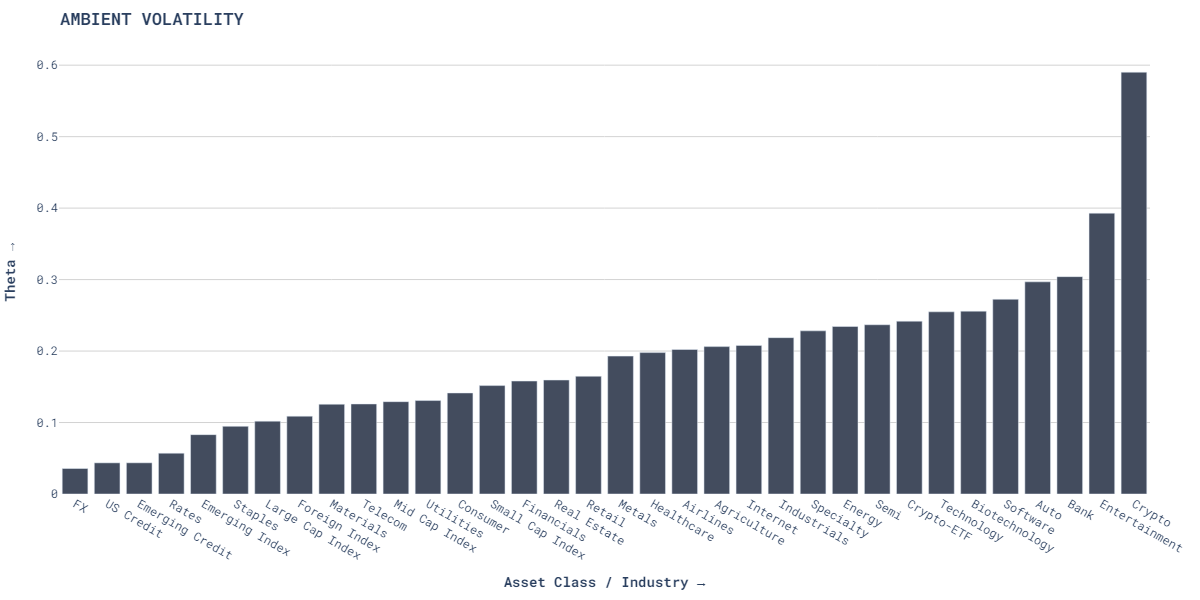
\includegraphics[width=\textwidth]{images/ambient_volatility_by_category.png}
    \caption{Ambient Volatility by Category}
    \label{fig:theta_by_category}
\end{figure}


The Cryptocurrencies which are deeply speculative in nature has an extraordinarily high ambient volatility compared to other asset classes. The entertainment industry which is mainly driven by consumer cyclicality seconds cryptocurrency in terms of long run volatility.
The sectors which are driven by innovation cycles and competitions such as technology biotechnology and automotive have relatively moderate ambient volatilities. The assets such as FX, Corporate and Treasury bonds  which are driven by macroeconomic factors such as interest rates, credit risks have the lowest levels of ambient volatility because their volatility are actively managed by central banks.


\subsubsection{ Mean Reversion $(\kappa)$}
The most interesting aspect of this kind of analysis is looking at the strength of mean reversion across tickers and asset classes.  The following chart shows the mean reversion rates as estimated by Ornestein-Ulhenback process aggregated for each sector. Although this chart is not very interpretable, therefore, in the next paragraph we modify the this mean reversion coefficient so as to look at expected time taken to reach the ambient volatility $(\theta)$ starting from a certain level of volatility. This helps to introduce interpretability in the mean reversion coefficient.

\begin{figure}[H]
    \centering
    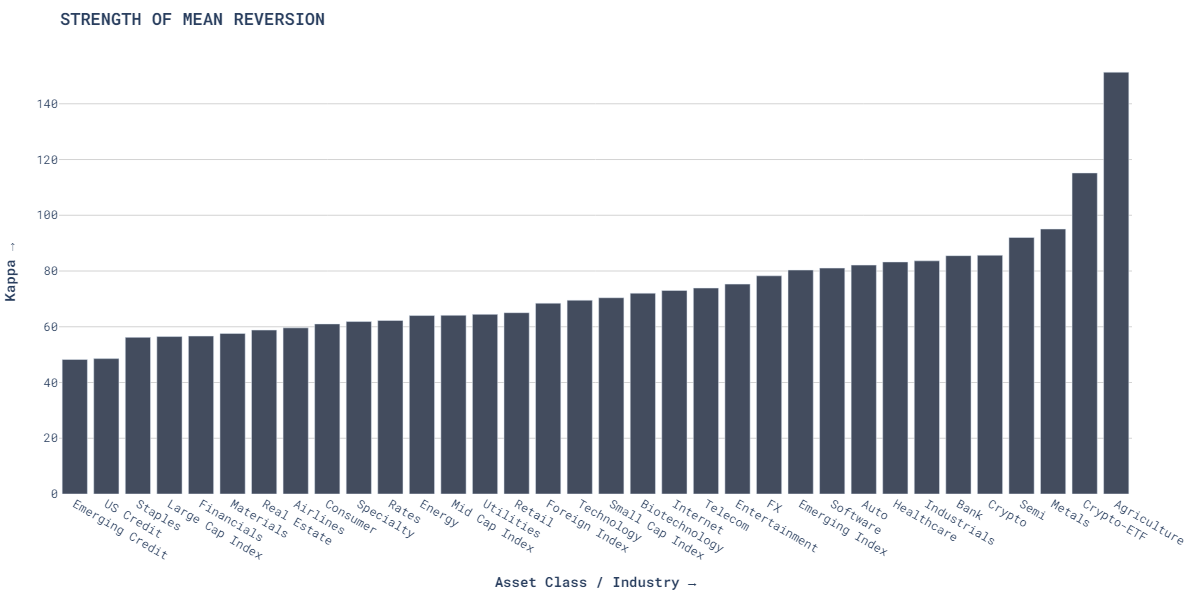
\includegraphics[width=\textwidth]{images/mean_reversion_by_category.png}
    \caption{Mean Reversion By Category}
    \label{fig:figure_label}
\end{figure}

Now since we know the mean reversion coefficient, we can ask another interesting question what is the expected amount of time it would take to reach from one level of volatility to another level of volatility. Since we have calibrated all the parameters of the stochastic differential equation, we can simulate different paths the volatility process could take which will enable us to look at the distribution of these Monte Carlo paths to estimate the parameter of interest.

To determine the expected amount of time that would elapse before the volatility touches its long run mean ($\theta$), we would first need to define, the first hitting or crossover time of the volatility process. Suppose we start from a volatility level $C$ and want to reach a volatility level of $A$. The expected time $T_{AC}$ can be expressed as an infimum over the set of all days $t$ where a single path crosses that volatility threshold.

$$ T_{A,C} = \inf\biggl\{ t\geq 0 \;: \; X_t = A \bigg| X_0 = C   \biggr\} $$

We can generate a large number of paths and the average of the infimums will give us the expected time to reach the level of ambient volatility.

To illustrate this concept, we can look at the iShares 20+ Year Treasury Bond ETF (TLT) which has a relatively slower mean reversion ($\kappa$) and we set the initial volatility level to be very high at 0.5, for the sake of a nice visualization. The estimated ambient volatility ($\theta$) of this ticker through Ornestien-Uhlenbeck process is 0.08. We generate 5000 Monte Carlo paths and we can observe that the volatility process is mean reverting to its ambient level over all the paths. To estimate the expected time to reach the ambient level, we take the average of the first crossovers over 5000 paths, which comes out to be 13.1 trading days with a standard error of 0.07 trading days.

\begin{figure}[H]
    \centering
    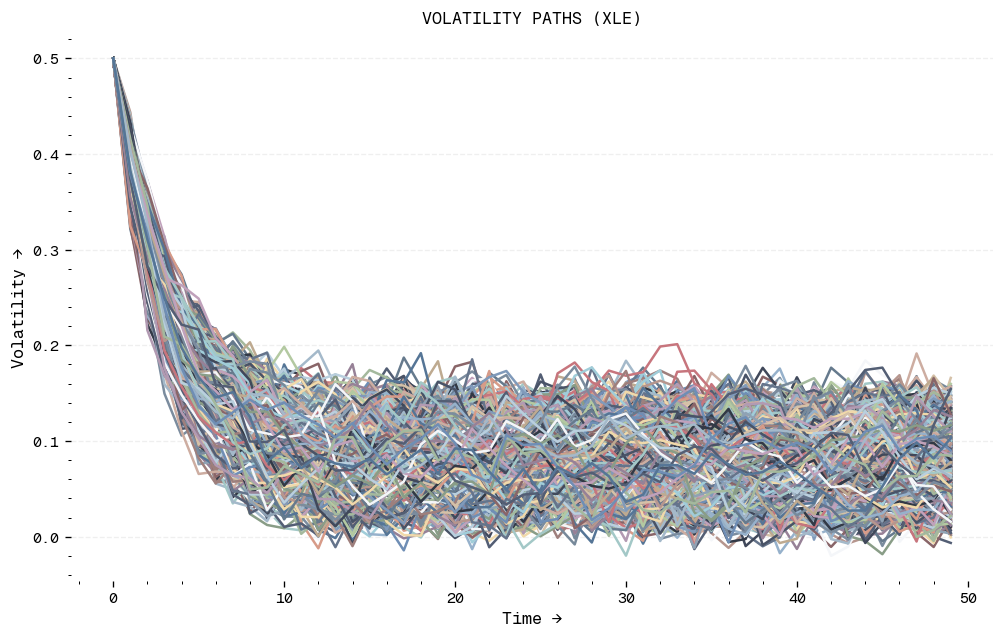
\includegraphics[width=\textwidth]{images/volatility_paths.png}
    \caption{Simulated 5000 paths of volatility process for TLT}
    \label{fig:figure_label}
\end{figure}

Please also note that very few volatility paths drop below zero. This is a Weiner process artefact and can be ignored, since we are looking at sufficiently large number of realizations.

A more interpretable version of looking at the mean reversion is to look at the expected number of days it will take for the volatility to reach its ambient level, given a starting level of volatility. The following chart shows the expected number of days it will take for the volatility to reach its ambient level ($\theta$) estimated through Ornestien-Uhlenbeck process for each industry / asset class, when we start from a pathologically high level of volatility of 0.5.

\begin{figure}[H]
    \centering
    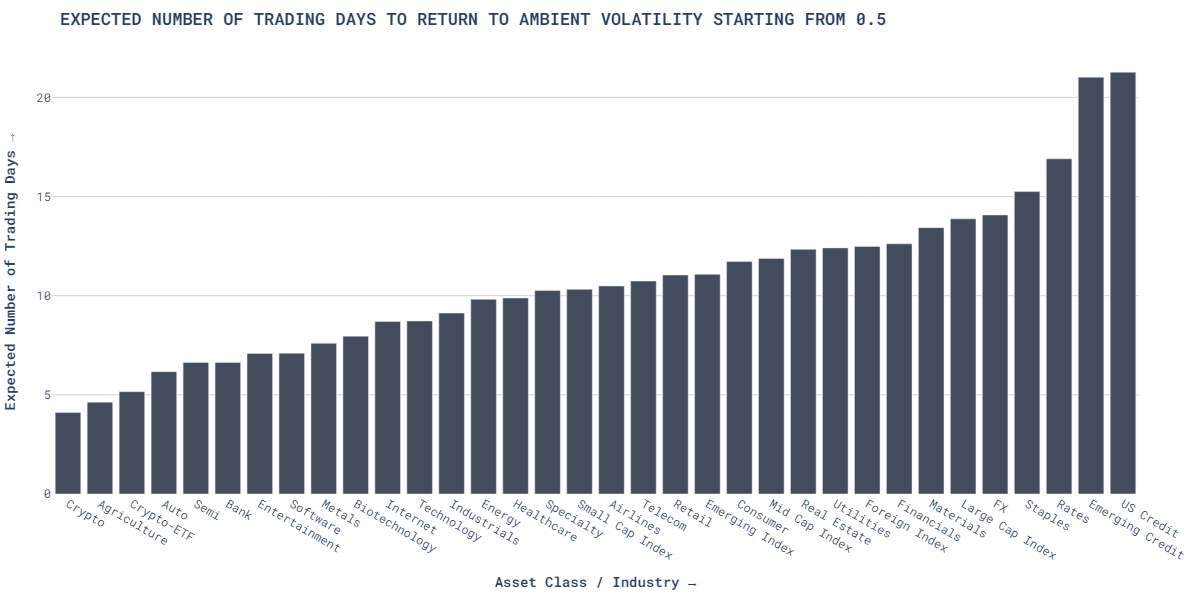
\includegraphics[width=\textwidth]{images/time_to_theta.png}
    \caption{Expected Time to Reach Ambient Volatility starting from a high volatility of 0.5}
    \label{fig:figure_label}
\end{figure}


If we start from a high volatility of 0.5, they take approximately four trading days to mean revert to their ambient volatility. A strong mean reversion tendency in agricultural tickers  is possibly due to the strong seasonal fluctuations inherent in these industries (\cite{Sorensen1999}). Cryptocurrency markets might be characterized by strong bursts of volatility which quickly stabilizes.

On the right end of the distribution, we have the industries that are highly sensitive to macroeconomic factors that influence credit markets such as Corporate bonds ETFs (HYG and LQD), Treasury Bond ETFs (TLT and IEF) of US and other emerging markets (EMB). These asset classes are heavily influenced by interest rates and default risks. Interest rate cycles usually span over several months and hence the volatility is expected to be persistent in these asset classes.

All the asset classes that relate to commodities and industrials like metal and energy sectors show reversion time around 6 to 8 trading days (starting from a high volatility) which indicates a relatively moderately persistent volatility.  The chart does not show the standard errors associated with each estimate of expected number of days however the standard error is extremely low possible because of a large sample realizations (5000 paths). The maximum standard error observed for the expected number of days over all tickers is one tenth of a trading day. The expected time levels as well as their associated standard errors for each ticker is shown in the appendix.

One more interesting insight emerges when we look at the scatter of the mean reversion against ambient volatility. 

\begin{figure}[H]
    \centering
    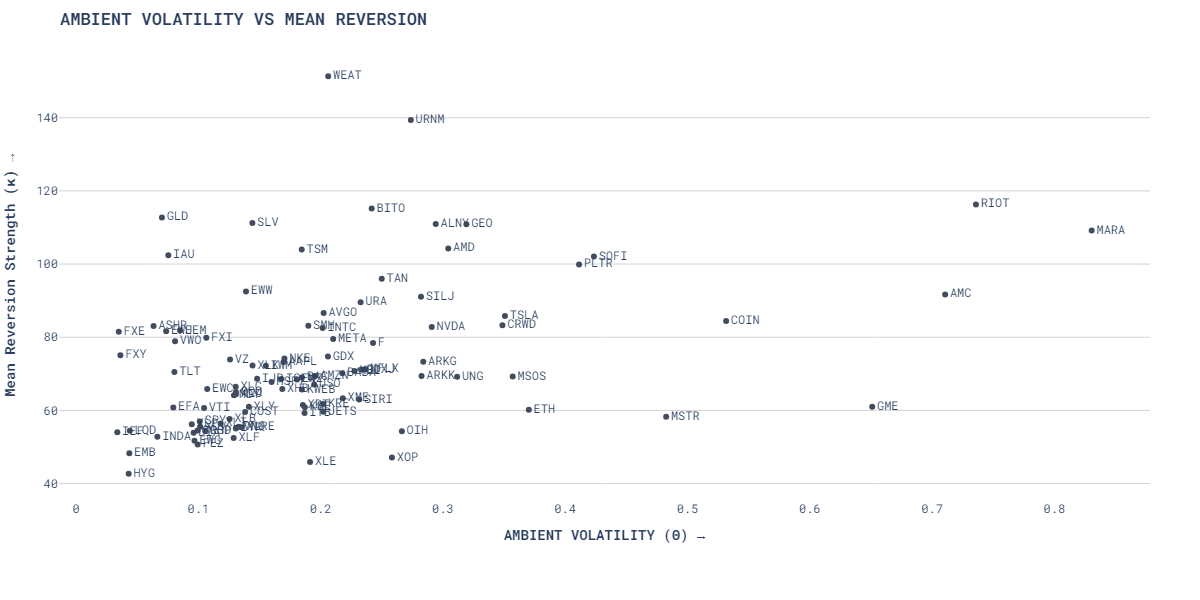
\includegraphics[width=\textwidth]{images/ambient_volatility_vs_mean_reversion.png}
    \caption{Scatter of Ambient Volatility vs Mean Reversion}
    \label{fig:figure_label}
\end{figure}

The strength of mean reversion has a heteroscedastic relationship with ambient volatility that is the variability of mean reversion across the cross section of tickers is conditional on what level of ambient volatility we are looking at.  At the lower levels of ambient volatility we find a strong visible correlation between the strength of mean reversion and ambient volatility which further dampens as we move to higher levels of ambient volatility across the cross section of tickers.



\subsubsection{ Meta Volatility $(\sigma)$  }

The meta volatility is the volatility of the volatility. The following chart shows the meta volatility as estimated by Ornestein-Ulhenback process aggregated for each industry / asset class.

\begin{figure}[H]
    \centering
    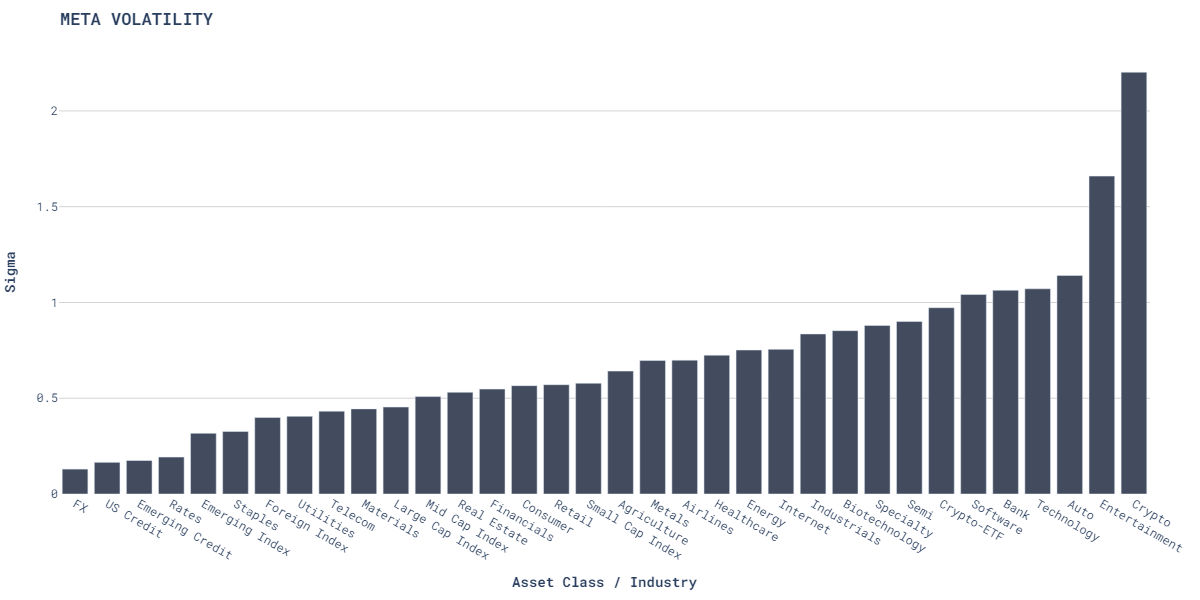
\includegraphics[width=\textwidth]{images/meta_volatility_by_category.png}
    \caption{Meta Volatility by Asset Class}
    \label{fig:figure_label}
\end{figure}

A truly interesting insight here is that this chart looks very similar to the ambient volatility chart in Figure \ref{fig:theta_by_category}. The empirical implication here is that if a asset class is characterized by a high level of ambient volatility, the volatility inherent in the ambient volatility is also high. This is apparently visible if we  look at the scatter of meta volatility against the ambient volatility.

\begin{figure}[H]
    \centering
    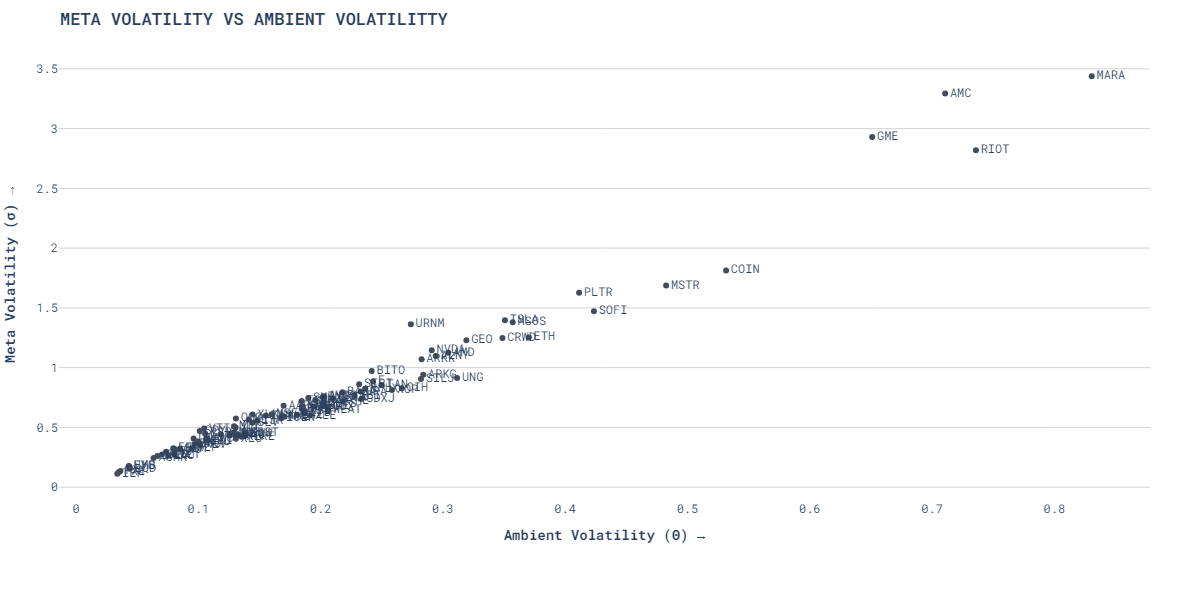
\includegraphics[width=\textwidth]{images/meta_volatility_vs_ambient_volatility.png}
    \caption{Scatter of Meta Volatility vs Ambient Volatility}
    \label{fig:figure_label}
\end{figure}

The relationship of meta volatility with the strength of mean reversion is similar to the relationship of ambient volatility with that of mean reversion. This is evident in the scatter below.

\begin{figure}[H]
    \centering
    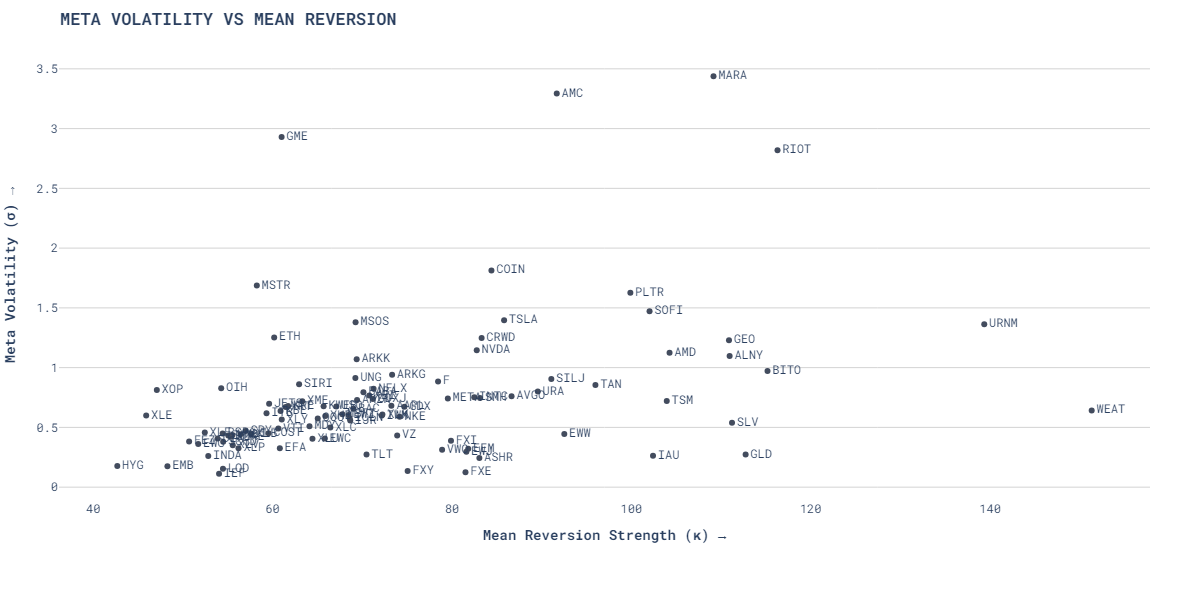
\includegraphics[width=\textwidth]{images/meta_volatility_vs_mean_reversion.png}
    \caption{Scatter of Meta Volatility vs Mean Reversion}
    \label{fig:figure_label}
\end{figure}

\section{ Roadmap from here}

\begin{displayquote}

“Forty-two!" yelled Loonquawl. "Is that all you've got to show for seven and a half million years' work?"  "I checked it very thoroughly," said the computer, "and that quite definitely is the answer. I think the problem, to be quite honest with you, is that you've never actually known what the question is.”  - Douglas Adams, The Hitchhiker’s Guide to the Galaxy

\end{displayquote}

Now I will venture into options market from the underlying spot markets.  The options market gives me two additional pieces of information that is the implied volatility and the skew.  At this point, I have a powerful model for the realised volatility.  This will enable me to ask good questions about  the implied volatility and the markup of the implied and the realised volatility that is the volatility risk premium.

\begin{enumerate}
\item Every trading day I can measure the distance between the realised volatility from the ambient volatility. The farther is the the realised volatility from the ambient volatility, it will be interesting to see how Volatility Risk Premium moves. Using these insights, can I find options that are mispriced or priced cheaply in the market?
\item I can use the gap between realised volatility and ambient volatility to see if market is overreacting to short term volatility bursts. This could be an incredibly useful trading signal.
\item Is the current implied volatility accurately pricing the future realized volatility? Is there a pattern when implied volatility consistently overshoots or underpredicts the future realised volatility.
\item I also know the mean reversion speed of the volatility process for each ticker. This can reveal potential mispricing of short term options.
\item How does the skew move with realized volatility?
\item How is skew distributed across asset classes?
\end{enumerate}


These questions would change and evolve as I move forward in the thesis. I am not sure, if I am still asking the right questions. The questions would themselves appear with the data. Motion creates information. Peace.






\printbibliography
\section{Appendix}
\subsection{Tickers and Asset Classes}

\begin{table}[H]
    \centering
    \small
    \begin{tabular}{ll}
        \toprule
        Ticker & Category \\   
        \midrule
        WEAT & Agriculture \\
        \hline
        JETS & Airlines \\
        \hline
        TSLA & Auto \\
        \hline
        F & Auto \\
        \hline
        BAC & Bank \\
        \hline
        SOFI & Bank \\
        \hline
        XBI & Biotechnology \\
        \hline
        ARKG & Biotechnology \\
        \hline
        XLY & Consumer \\
        \hline
        RIOT & Crypto \\
        \hline
        MSTR & Crypto \\
        \hline
        COIN & Crypto \\
        \hline
        MARA & Crypto \\
        \hline
        ETH & Crypto \\
        \hline
        BITO & Crypto-ETF \\
        \hline
        EMB & Emerging Credit \\
        \hline
        VWO & Emerging Index \\
        \hline
        EEM & Emerging Index \\
        \hline
        ICLN & Energy \\
        \hline
        XLE & Energy \\
        \hline
        XOP & Energy \\
        \hline
        USO & Energy \\
        \hline
        TAN & Energy \\
        \hline
        OIH & Energy \\
        \hline
        UNG & Energy \\
        \hline
        NFLX & Entertainment \\
        \hline
        AMC & Entertainment \\
        \hline
        SIRI & Entertainment \\
        \hline
        XLF & Financials \\
        \hline
        KBE & Financials \\
        \hline
        INDA & Foreign Index \\
        \hline
        EWJ & Foreign Index \\
        \hline
        KWEB & Foreign Index \\
        \hline
        FXI & Foreign Index \\
        \hline
        EWC & Foreign Index \\
        \hline
        EWG & Foreign Index \\
        \hline
        EWZ & Foreign Index \\
        \hline
        FEZ & Foreign Index \\
        \hline
        EWW & Foreign Index \\
        \hline
        ASHR & Foreign Index \\
        \hline
        EFA & Foreign Index \\
        \hline
        FXY & FX \\
        \hline
        FXE & FX \\
        \hline
        XLV & Healthcare \\
        \hline
        ALNY & Healthcare \\
        \hline
        XLI & Industrials \\
        \hline
        GEO & Industrials \\
        \hline
        AMZN & Internet \\
        \hline
        BABA & Internet \\
        \hline
        META & Internet \\
        \hline
        DIA & Large Cap Index \\
        \hline
        RSP & Large Cap Index \\
        \hline
        VTI & Large Cap Index \\
        \hline
        SPY & Large Cap Index \\
        \hline
        XLB & Materials \\
        \hline
        SILJ & Metals \\
        \hline
        GDXJ & Metals \\
        \hline
        XME & Metals \\
        \hline
        URNM & Metals \\
        \hline
        GDX & Metals \\
        \hline
        URA & Metals \\
        \hline
        GLD & Metals \\
        \hline
        IAU & Metals \\
        \hline
        SLV & Metals \\
        \hline
        MDY & Mid Cap Index \\
        \hline
        TLT & Rates \\
        \hline
        IEF & Rates \\
        \hline
        ITB & Real Estate \\
        \hline
        XHB & Real Estate \\
        \hline
        IYR & Real Estate \\
        \hline
        XLRE & Real Estate \\
        \hline
        KRE & Real Estate \\
        \hline
        VNQ & Real Estate \\
        \hline
        XRT & Retail \\
        \hline
        COST & Retail \\
        \hline
        NKE & Retail \\
        \hline
        AVGO & Semi \\
        \hline
        AMD & Semi \\
        \hline
        TSM & Semi \\
        \hline
        INTC & Semi \\
        \hline
        NVDA & Semi \\
        \hline
        IJR & Small Cap Index \\
        \hline
        IWM & Small Cap Index \\
        \hline
        CRWD & Software \\
        \hline
        MSFT & Software \\
        \hline
        AAPL & Software \\
        \hline
        PLTR & Software \\
        \hline
        SCHD & Specialty \\
        \hline
        MSOS & Specialty \\
        \hline
        XLP & Staples \\
        \hline
        SMH & Technology \\
        \hline
        ARKK & Technology \\
        \hline
        QQQ & Technology \\
        \hline
        XLK & Technology \\
        \hline
        GME & Technology \\
        \hline
        XLC & Technology \\
        \hline
        VZ & Telecom \\
        \hline
        HYG & US Credit \\
        \hline
        LQD & US Credit \\
        \hline
        XLU & Utilities \\
        \bottomrule
        \end{tabular}      
    \label{table:tickers}
\end{table}

\end{document}